\subsection{Problems for Developers} \label{subsection:foundation-piracy-developers}
Piracy is a big problem for developers as seen in figure~\ref{fig:revenue}.
The developer loses direct revenue when his \gls{ip} is stolen and redistributed by a pirate without the developer's involvement.
In case the application is offered for free, users do not have to pay and no revenue is generated.
It is even worse when the pirated application is sold in another application store.
In this case the pirate gets the profit which should be the developer's.
\newline
Revenue is not only lost when the application can be downloaded for free.
There is also follow up revenue effected, when an applications is changed.
There are two main types of indirect revenue.
\newline
The first type is in-app purchases.
They are a popular source of income for so called freemium or lite versions of  application lications.
In case of the the freemium app, the download is for free and includes all features.
The developer makes the money with in-app purchases like cosmetic interface changes or in-game currency.
The lite version application is a little bit different.
The download is free as well, but the application comes with a restricted feature set or limited time of use.
In order to take advantage of the full feature set, the user can buy the pro-license via an in-app purchase.
\newline
Apps can include a mix or various degrees of theses types.
Pirates can disable the transaction of the payments for in-app purchase thus no earnings are generated for the developer while the user can access the content.
\newline
The second type of indirect revenue is generated by showing in-app advertisements.
When this feature is implemented, advertisements are shown inside the application and the developer is paid by views and clicks on the advertisements.
Commissions earned this way are assigned according to the Ad Unit ID \cite{googleAdmob} stored in the application.
When an application is pirated, this ID can be replaced by the pirate's ID and commissions funneled to the pirate.
\newline
\begin{figure}[h]
    \centering
    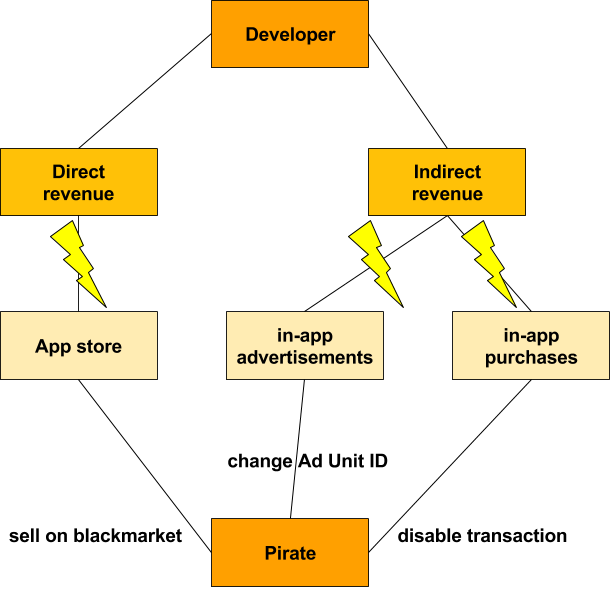
\includegraphics[width=0.8\textwidth]{data/revenue.png}
    \caption{Different ways to generate revenue and how the pirate can cut them}
    \label{fig:revenue}
\end{figure}
\newline
Beside monetary issues, additional problems arise when the application is moved to a black market store or website and then distributed without the environment of an official application store.
This results is the loss of control over the application for the developer.
He can no longer provide support and updates for the application.
The users will not get fixes for security issues and bugs.
Users which do not know they are using a pirated version will connect the unsatisfying behavior to the developer.
This results in the loss of reputation and potential future revenues not even connected to original application.
\newline
If an application uses server resources, the developer can neither monitor the growth in the usage of their application nor do they get the money to upgrade it \cite{lierschDeveloperThreats}.
\newline
Developers make a living of their applications.
When they do not make a profit, or even lose money with their servers, they can no longer continue.
The result is a loss of creativity, ideas and skills for the ecosystem.
